\documentclass[paper,onecolumn,twoside]{geophysics}

\usepackage{amsfonts}
\usepackage{amsmath}
\usepackage{dsfont}

% An example of defining macros
\newcommand{\rs}[1]{\mathstrut\mbox{\scriptsize\rm #1}}
\newcommand{\rr}[1]{\mbox{\rm #1}}

\newcommand{\citensp}[1]{\hspace{1sp}\cite{#1}}
\newcommand{\bs}[1]{\boldsymbol{#1}}
\newcommand{\R}{\mathbb{R}}

\begin{document}

\title{Optimal Transport for Seismic Source Inversion}

\renewcommand{\thefootnote}{\fnsymbol{footnote}} 

\address{
\footnotemark[1] Oden Institute, 
The University of Texas at Austin}
\author{Tyler Masthay\footnotemark[1] and Bj\"{o}rn Engquist\footnotemark[1]}

%\footer{Example}
%\lefthead{Dellinger \& Fomel}
%\righthead{\emph{Geophysics} example}

%\maketitle is unneccessary

\begin{abstract}
Full-waveform inversion (FWI) is a state-of-the-art method for imaging the earth's subsurface. However, FWI is notorious for local-minimum trapping, or ``cycle skipping,'' and thus requires an accurate initial model (\citensp{metivier2018optimal}).
Cycle skipping is caused by the nonconvex nature of the misfit optimization landscape in its typical least-squares formulation.
The Wasserstein-2 distance is convex with respect to shifts and dilations, both of which occur naturally in seismic data. Therefore, we propose using this optimal transport metric as our misfit for FWI. 
Previous work using optimal transport for source inversion, whose applications include microseismic event detection and deformation mechanics in subduction zones, has shown promise (\citensp{chen2018quadratic}). However, this work uses the acoustic wave equation, which is less accurate than the elastic wave equation.
In this paper, we extend these results to elastic source inversion in two spatial dimensions and show that they translate well to the elastic model.
\end{abstract}

\section{Introduction}
FWI is formulated as a PDE-constrained optimization problem with respect to a given misfit functional. Given that time shifts and amplitude dilations occur naturally in seismic data, we would ideally use a misfit functional that is convex with respect to these transformations. The Wasserstein-2 distance, denoted $W_2$, satisfies this property, whereas the industry standard $L^2$ misfit does not (\citensp{yang2018analysis}). 
$W_2(f,g)$ for probability densities $f,g$ on $X=\mathbb{R}^{n}$ is given by
\begin{align} \label{eqn:w2}
    W_2^2(f,g) := \inf_{T \in \mathcal{M}} \int_{X} |\bs{x} - T(\bs{x})|^2 f(\bs{x}) d\bs{x},
\end{align}
where $\mathcal{M}$ is the set of feasible transport maps (\citensp{villani2021topics}). $T$ transforms $g$ into the shape of $f$ in such a way that mass is preserved. That is, $T \in \mathcal{M}$ whenever for all closed rectangles $R \subseteq \mathbb{R}^{n}$
\begin{align*}
    \int_{\R} g(T(\bs{x})) det(\nabla T(\bs{x})) d\bs{x} = \int_{\R} f(\bs{x}) d\bs{x}.
\end{align*}

%\textcolor{red}{One difficulty of using this optimal-transport metric is that the distance is only defined between probability distributions. We thus renormalize our seismic data into probability distributions prior to using the Wasserstein distance.}
$W_2$ is defined between probability distributions, but seismic data are not probability distributions. 
Thus, we must renormalize our seismic data via some map $\mathcal{R}$. Many renormalization maps are explored in [\citensp{engquist2020optimal}]. An example is positive/negative splitting renormalization given by
\begin{align}\label{eqn:w2tilde}
    \tilde{W}_{2}^{2}(f,g) = W_{2}^{2}\left( \frac{f^{+}}{\|f^{+}\|_{L^1}}, \frac{g^{+}}{\|g^{+}\|_{L^1}}\right) + W_{2}^{2}\left(\frac{f^{-}}{\|f^{-}\|_{L^1}}, \frac{g^{-}}{\|g^{-}\|_{L^1}}\right),
\end{align}
where $F^{+}(x) = max(F(x), 0)$, $F^{-}(x) = max(-F(x), 0)$, and for given function $\phi$,
\begin{align*}
    \|\phi\|_{L^1} = \int_{\R} |\phi(x)| dx
\end{align*}
Figure \ref{fig:ricker-madagascar} demonstrates that convexity of $W_2$ under shift is preserved after renormalization of a model elastic wave with a Ricker wavelet source. Directly computing the $L^2$ norm clearly results in a nonconvex optimization landscape. Previous work has applied optimal transport to velocity and source inversion but has used the acoustic wave equation as the forward model (\citensp{chen2018quadratic},\cite{yang2018application}). In this paper, we apply optimal transport to seismic source inversion but with the elastic wave equation, a more complete and accurate forward model. We exhibit that the promising results from the acoustic model translate well to the elastic model. 

%I have another figure in Python that looks better than districker0.pdf
%    -- unsure why this plot does not seem to look as good
%\begin{figure}
%\includegraphics[width=0.5\textwidth]{Fig/w2.pdf}
%\includegraphics[width=0.5\textwidth]{Fig/l2.pdf}
%\caption{Comparison of optimization landscape of $W_2$ and $L^2$ distances for elastic waves that have been shifted away from origin according to varying $P$ and $S$-wave velocity differences.}
%\label{fig:ricker}
%\end{figure}

\begin{figure}
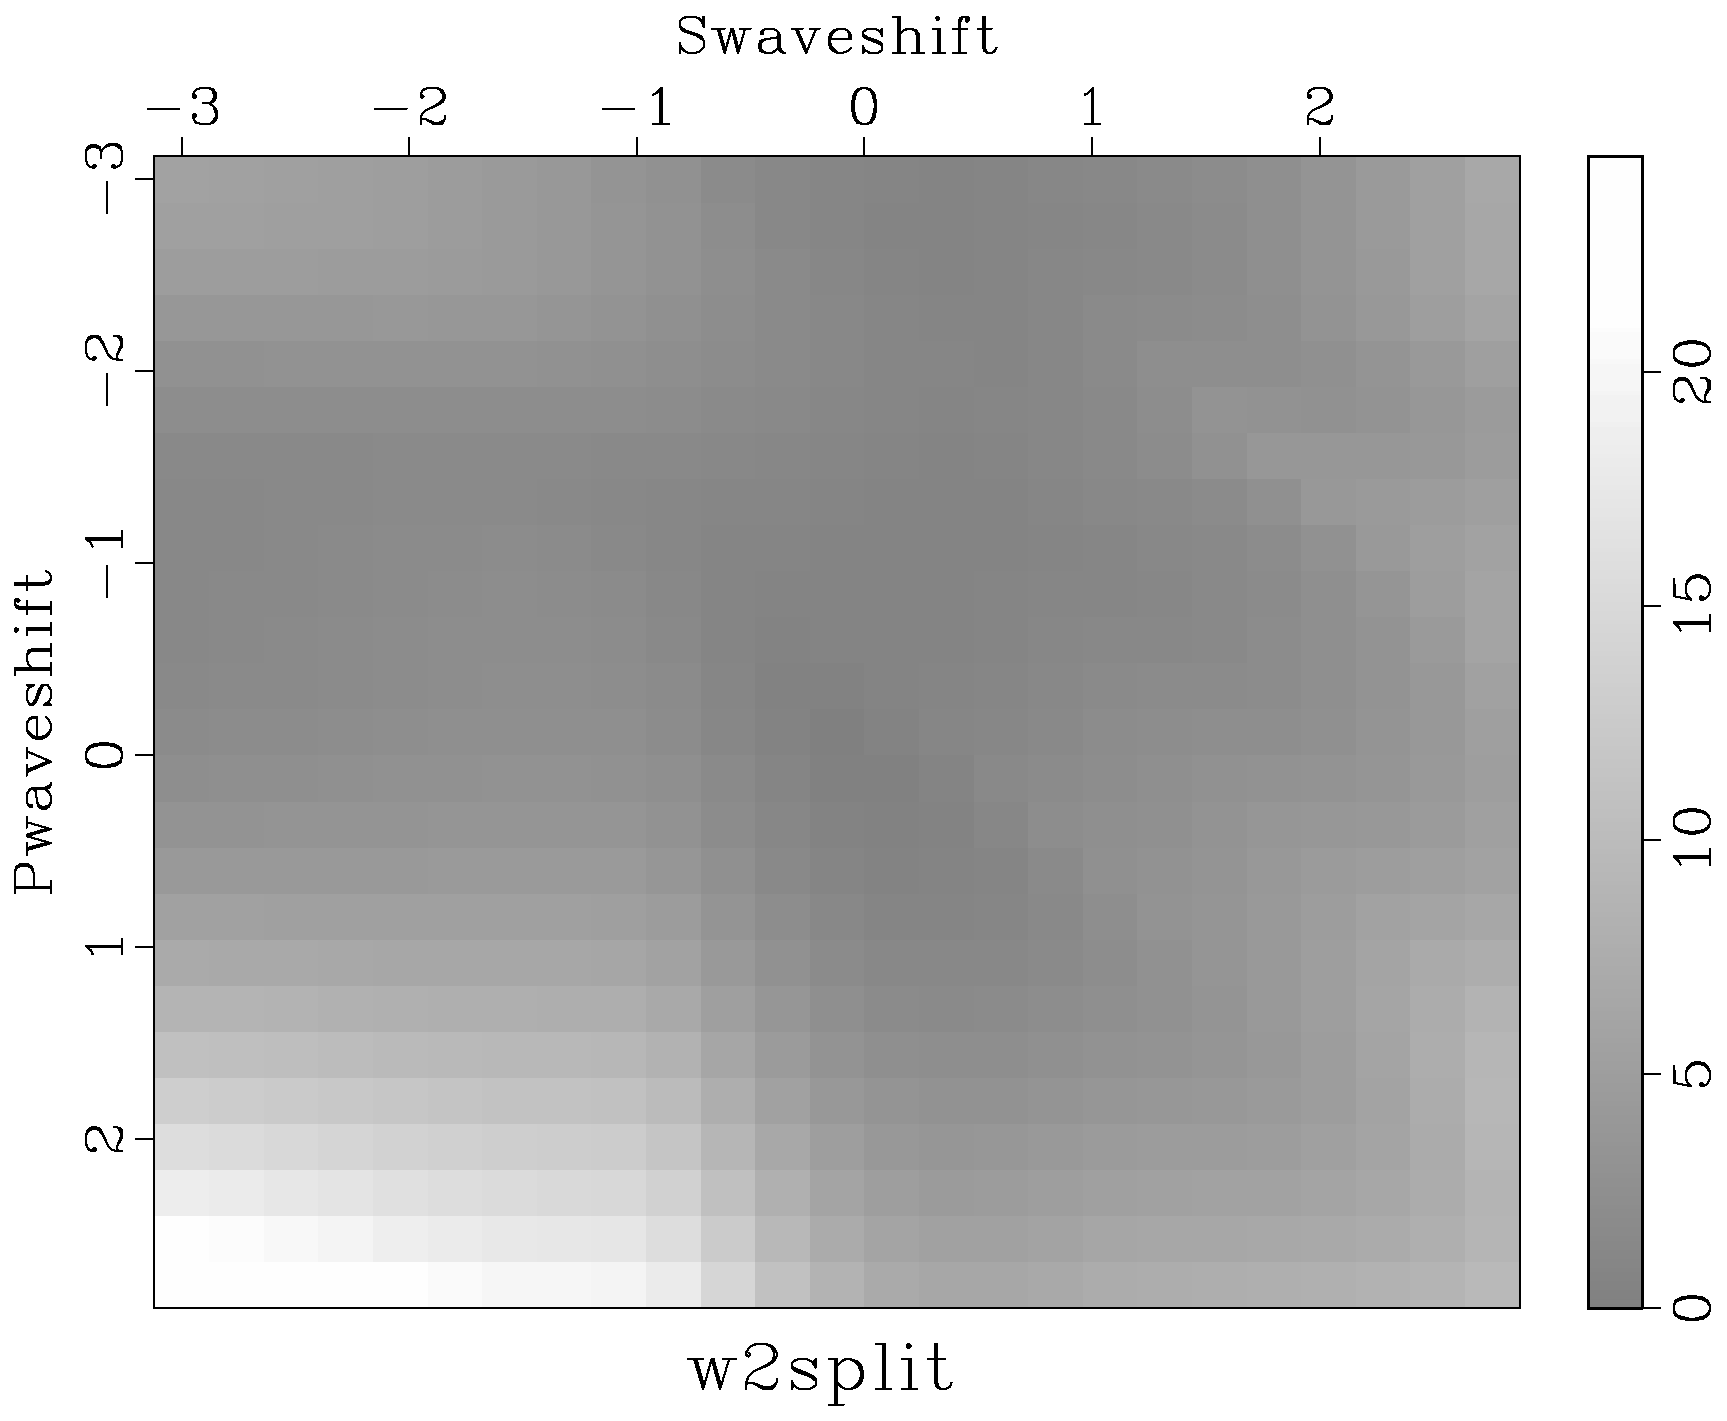
\includegraphics[width=0.5\textwidth]{Fig/districker0.pdf}
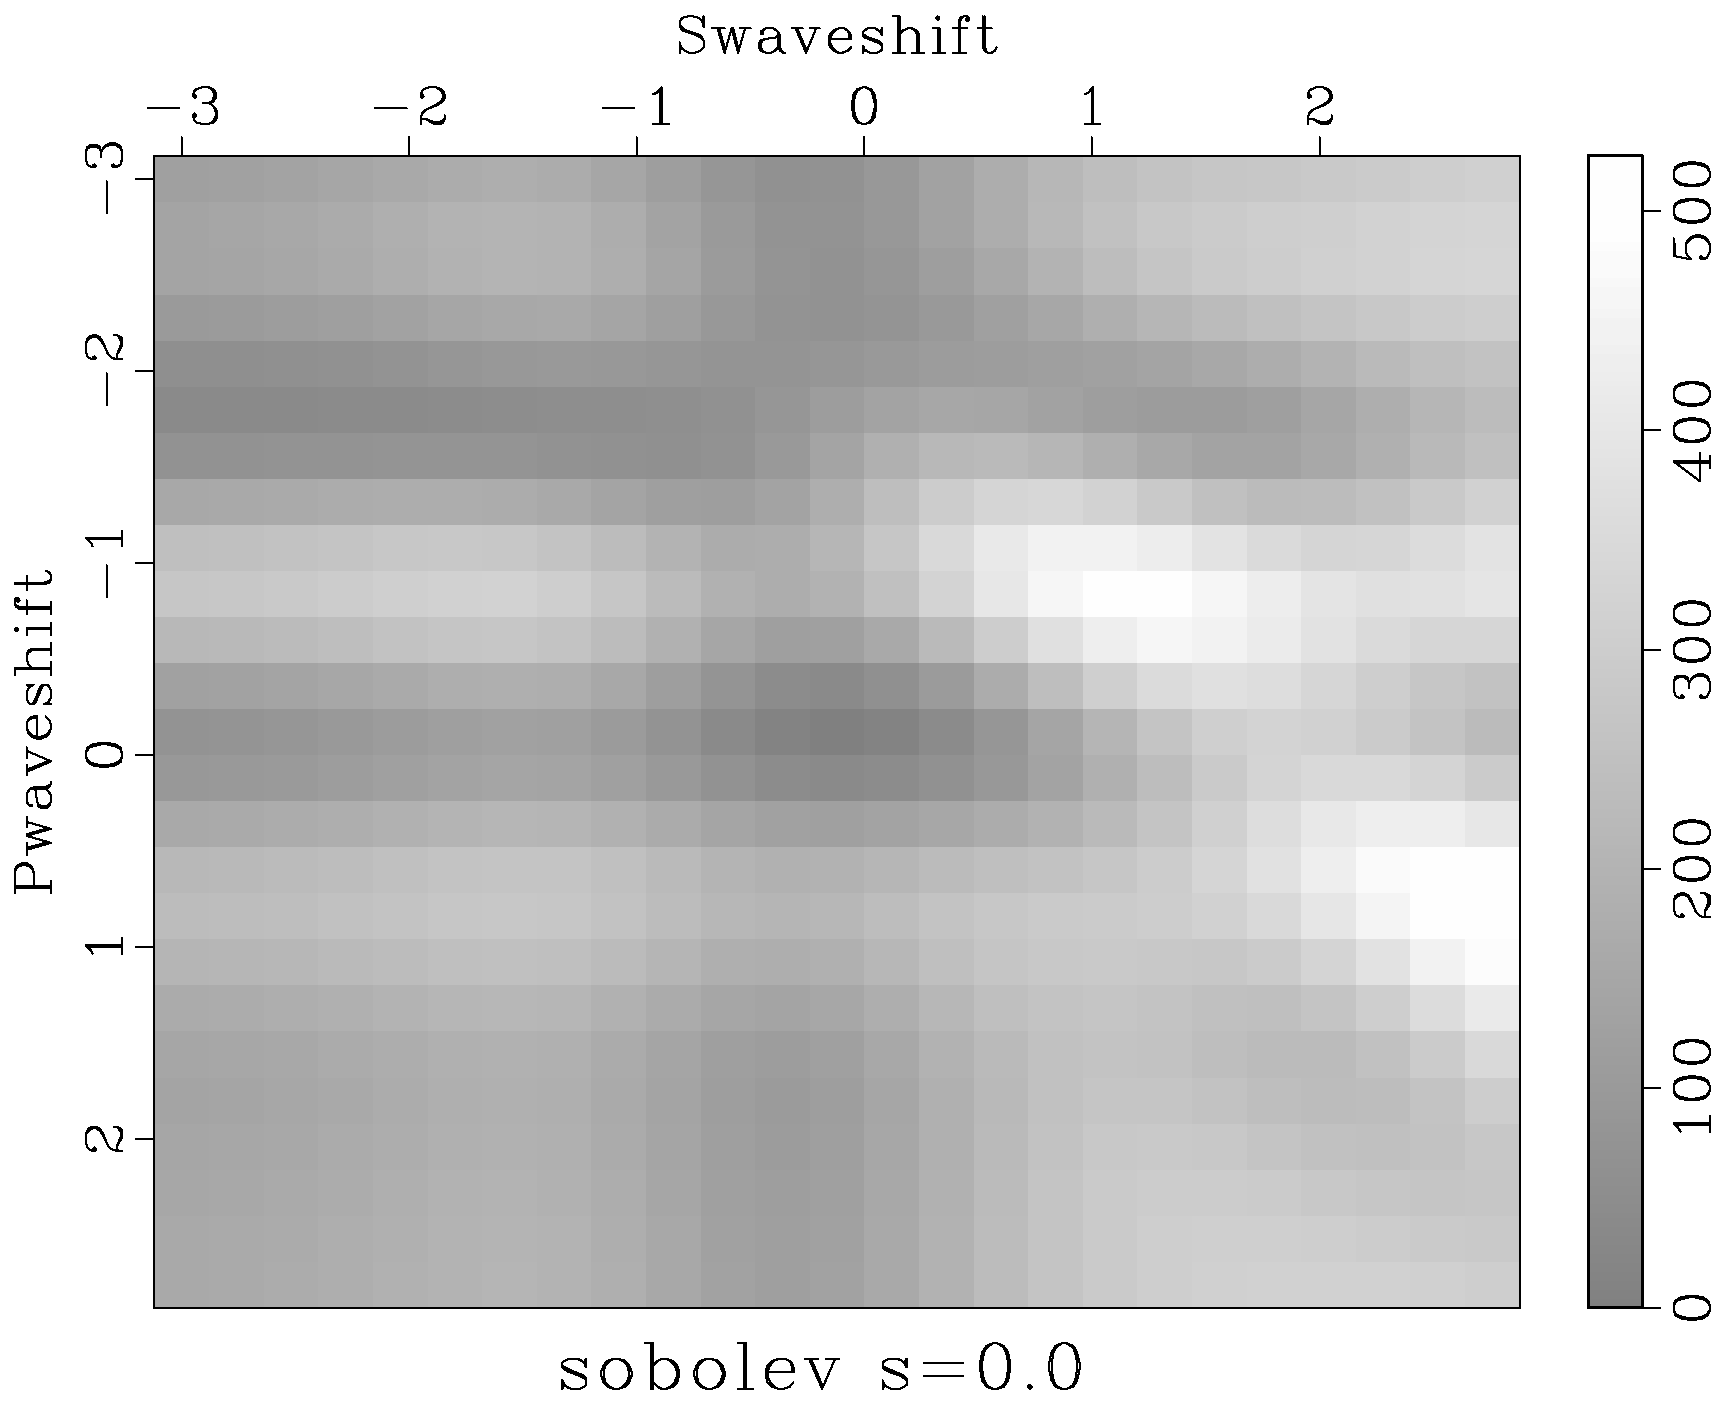
\includegraphics[width=0.5\textwidth]{Fig/districker1.pdf}
\caption{Comparison of optimization landscape of $W_2$ and $L^2$ distances for elastic waves that have been shifted away from origin according to varying $P$ and $S$-wave velocity differences.}
\label{fig:ricker-madagascar}
\end{figure}


\section{Results for IASP-91 Model}
The IASP-91 model is an approximation for P-wave and S-wave velocities to a depth of approximately $7000$ km. The model is a globally-averaged, one-dimensional model for the velocity fields and thus does not vary laterally. We approximate this model as a series of horizontal reflections to generate a realistic synthetic model. The velocity fields are shown in Figure \ref{fig:iaspvel}. Figure \ref{fig:iaspopt} compares the optimization landscapes for $L^2$ to $W_2$ with various renormalization methods. For this example, we generate synthetic data by setting a source in the center of the domain, so all misfits have a global optimum at the center of the domain. In addition to splitting, we tested (a) squaring renormalization, (b) linear renormalization, (c) exponential renormalization, and (d) ``linear exponential'' renormalization, i.e., a linear combination of (c) and (d). Squaring renormalization is given by
\begin{align} \label{eqn:square}
f \mapsto \frac{f^2}{\|f^2\|_{L^1}}.
\end{align}
Linear renormalization is given by
\begin{align} \label{eqn:linear}
f \mapsto \frac{f+c}{\|f+c\|_{L^1}}
\end{align}
for some $c$ such that $f + c \geq 0$.
Exponential renormalization is given by
\begin{align} \label{eqn:exponential}
f \mapsto \frac{exp(c f)}{\|exp(c f)\|_{L^1}}.
\end{align}
Finally, linear exponential renormalization
\begin{align} \label{eqn:linexp}
f \mapsto C_{c,f} \left( (f+\frac{1}{c})\mathds{1}_{\{f \geq 0\}} + \frac{1}{c} exp(c f) \mathds{1}_{\{f < 0\}}\right)
\end{align}
where $C_{c,f}$ is the appropriate normalization constant and $\mathds{1}$ is the indicator function. In our tests, we found that squaring and exponential renormalization worked the best. Linear and linear exponential seemed to corrupt the landscape significantly with the global minimum not being located in the center of the domain. However, we note that the optimization landscape for $W_2$ seems to be less sensitive to the depth of the source than $L^2$. This may be caused by the renormalization operation destroying amplitude information and suggests that further work should seek to rectify this loss of information.
\begin{figure}
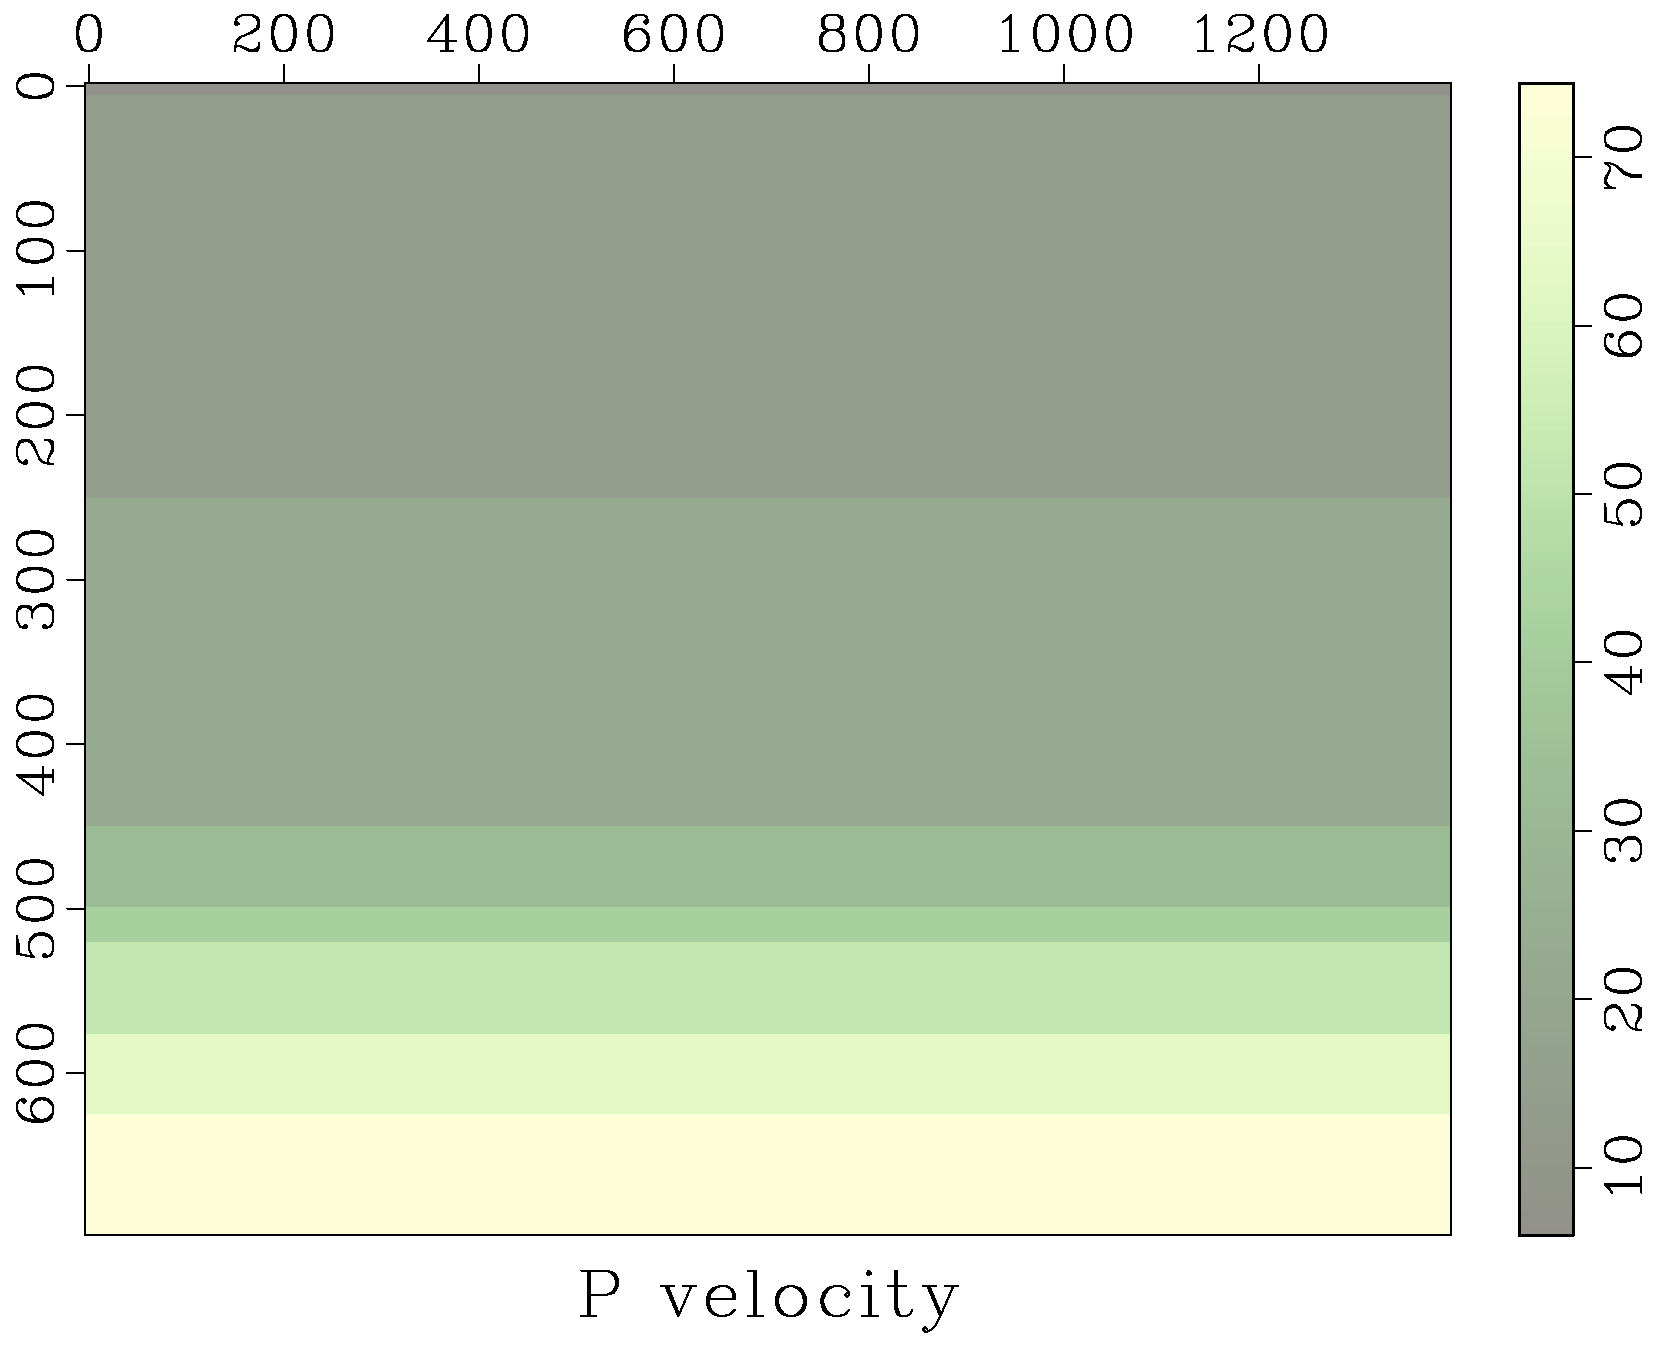
\includegraphics[width=0.5\textwidth]{Fig/vp.pdf}
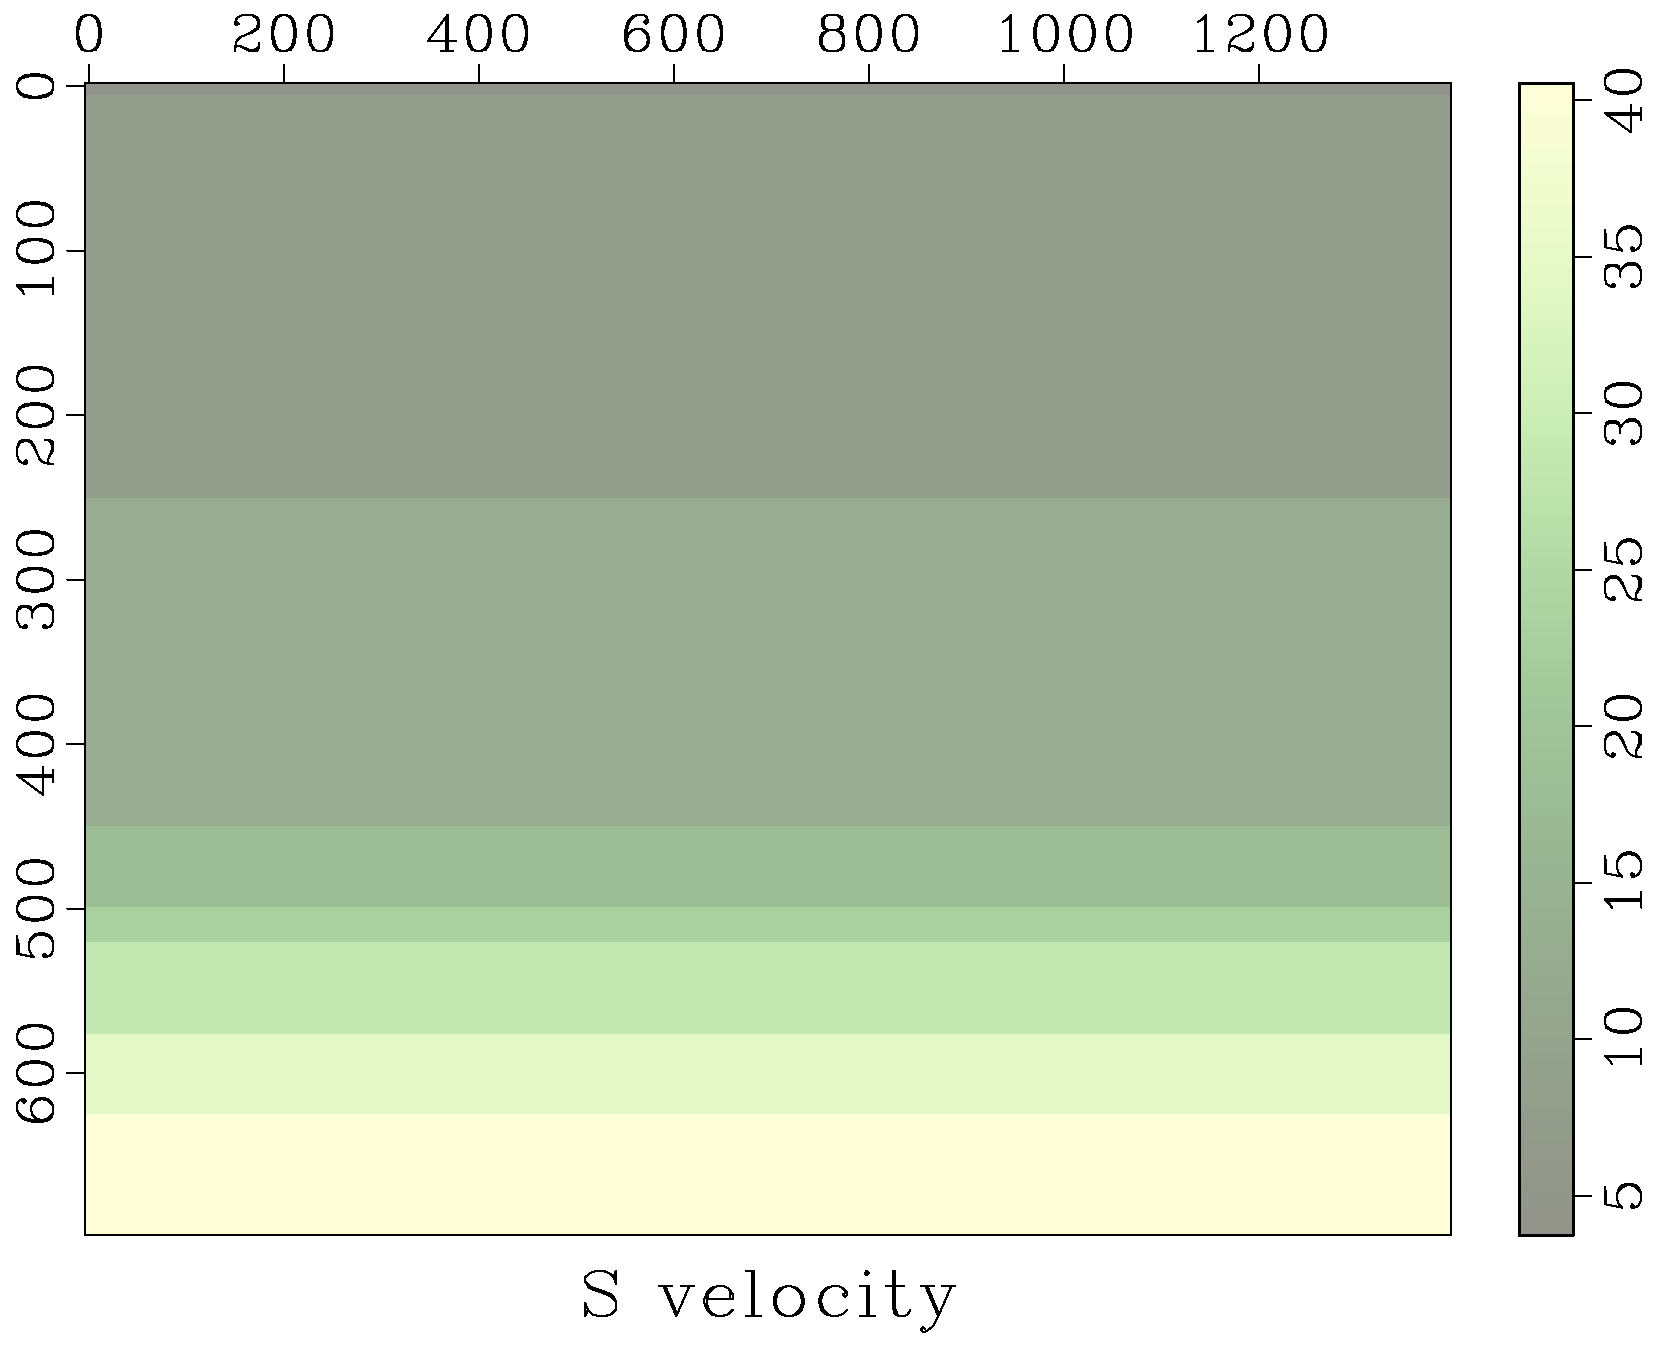
\includegraphics[width=0.5\textwidth]{Fig/vs.pdf}
\caption{P-wave and S-wave velocities for IASP-91 model}
\label{fig:iaspvel}
\end{figure}

\begin{figure}
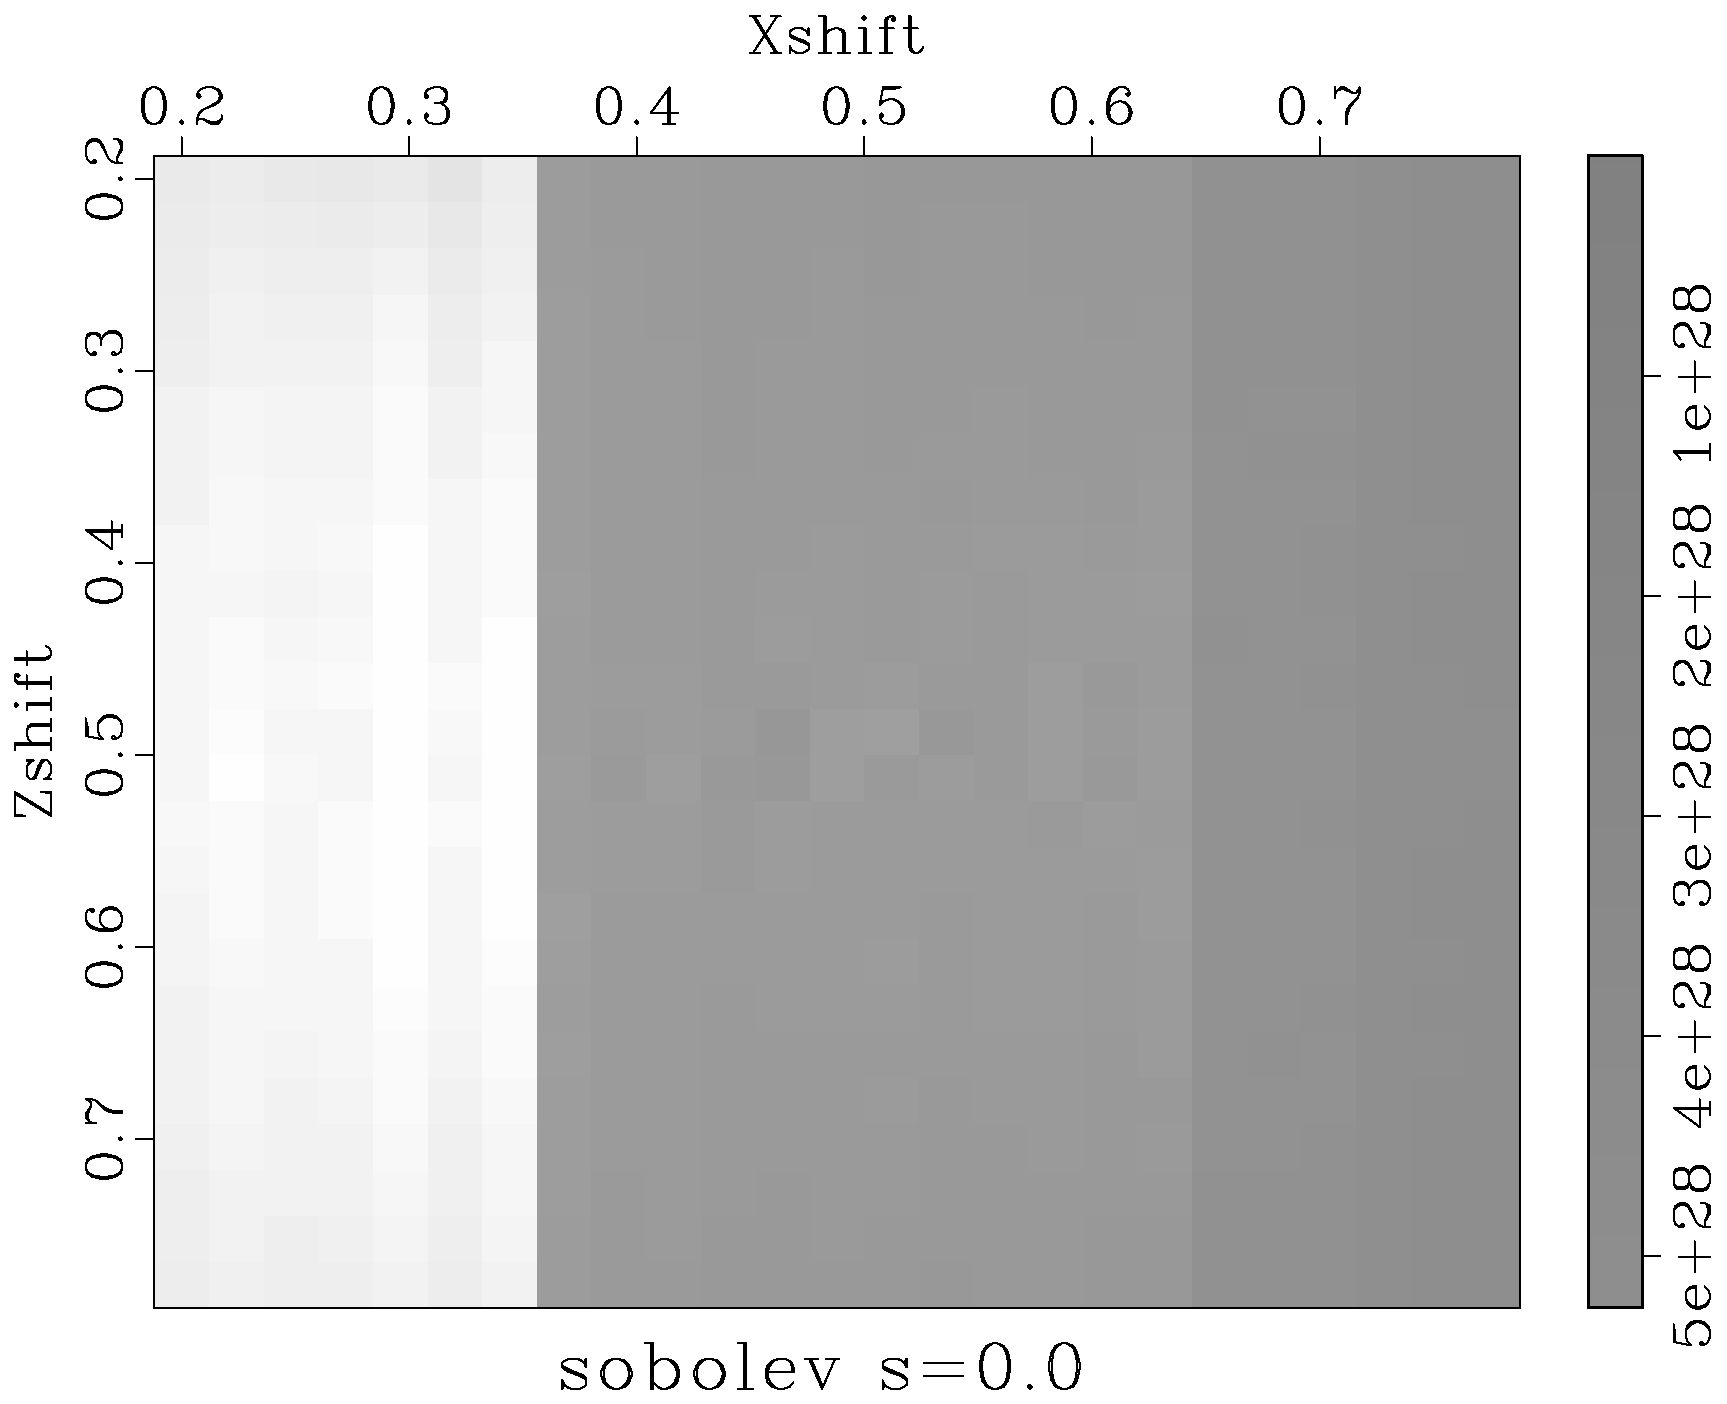
\includegraphics[width=0.5\textwidth]{Fig/fulldist0.pdf}
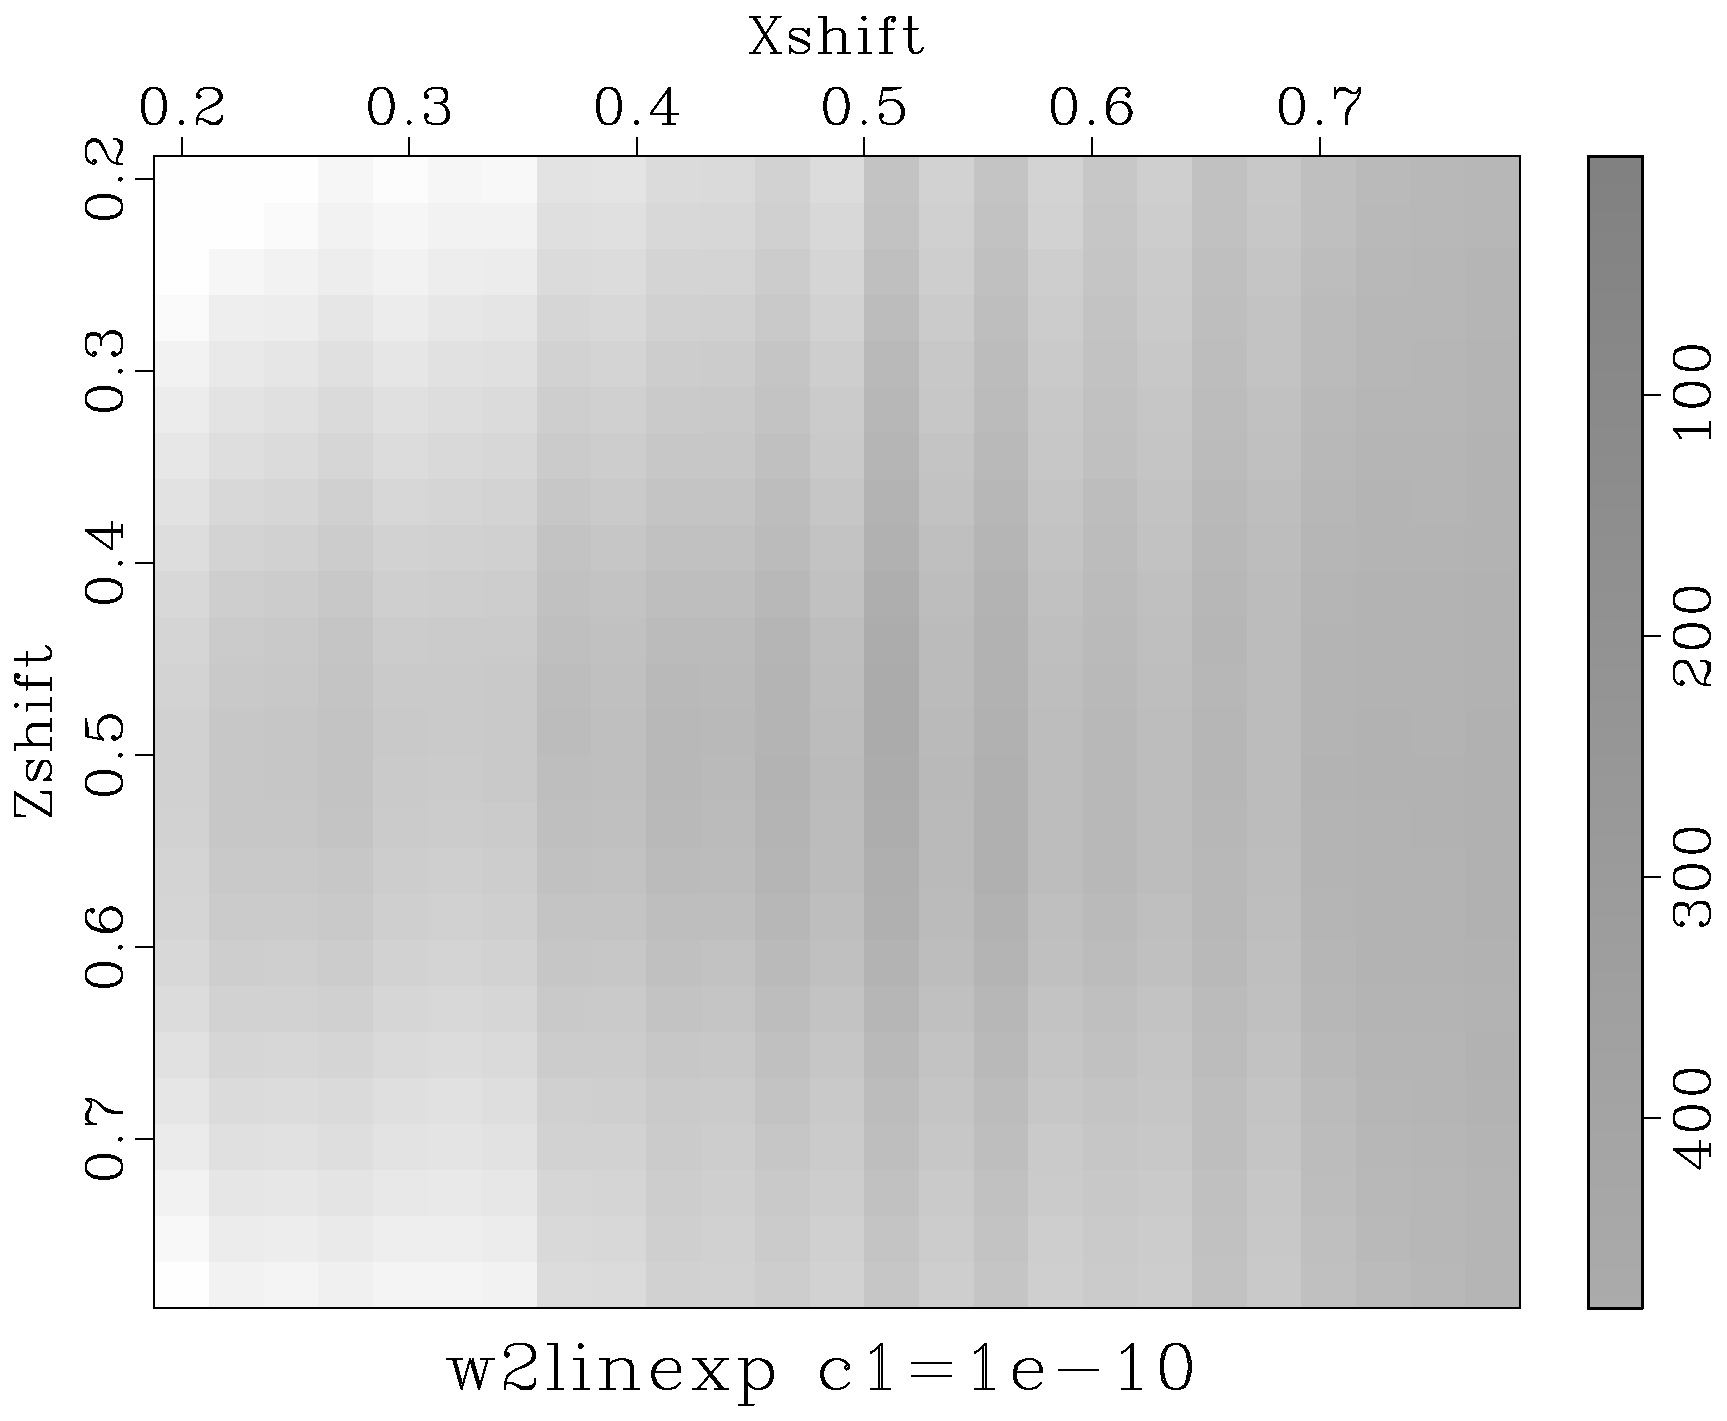
\includegraphics[width=0.5\textwidth]{Fig/fulldist1.pdf}
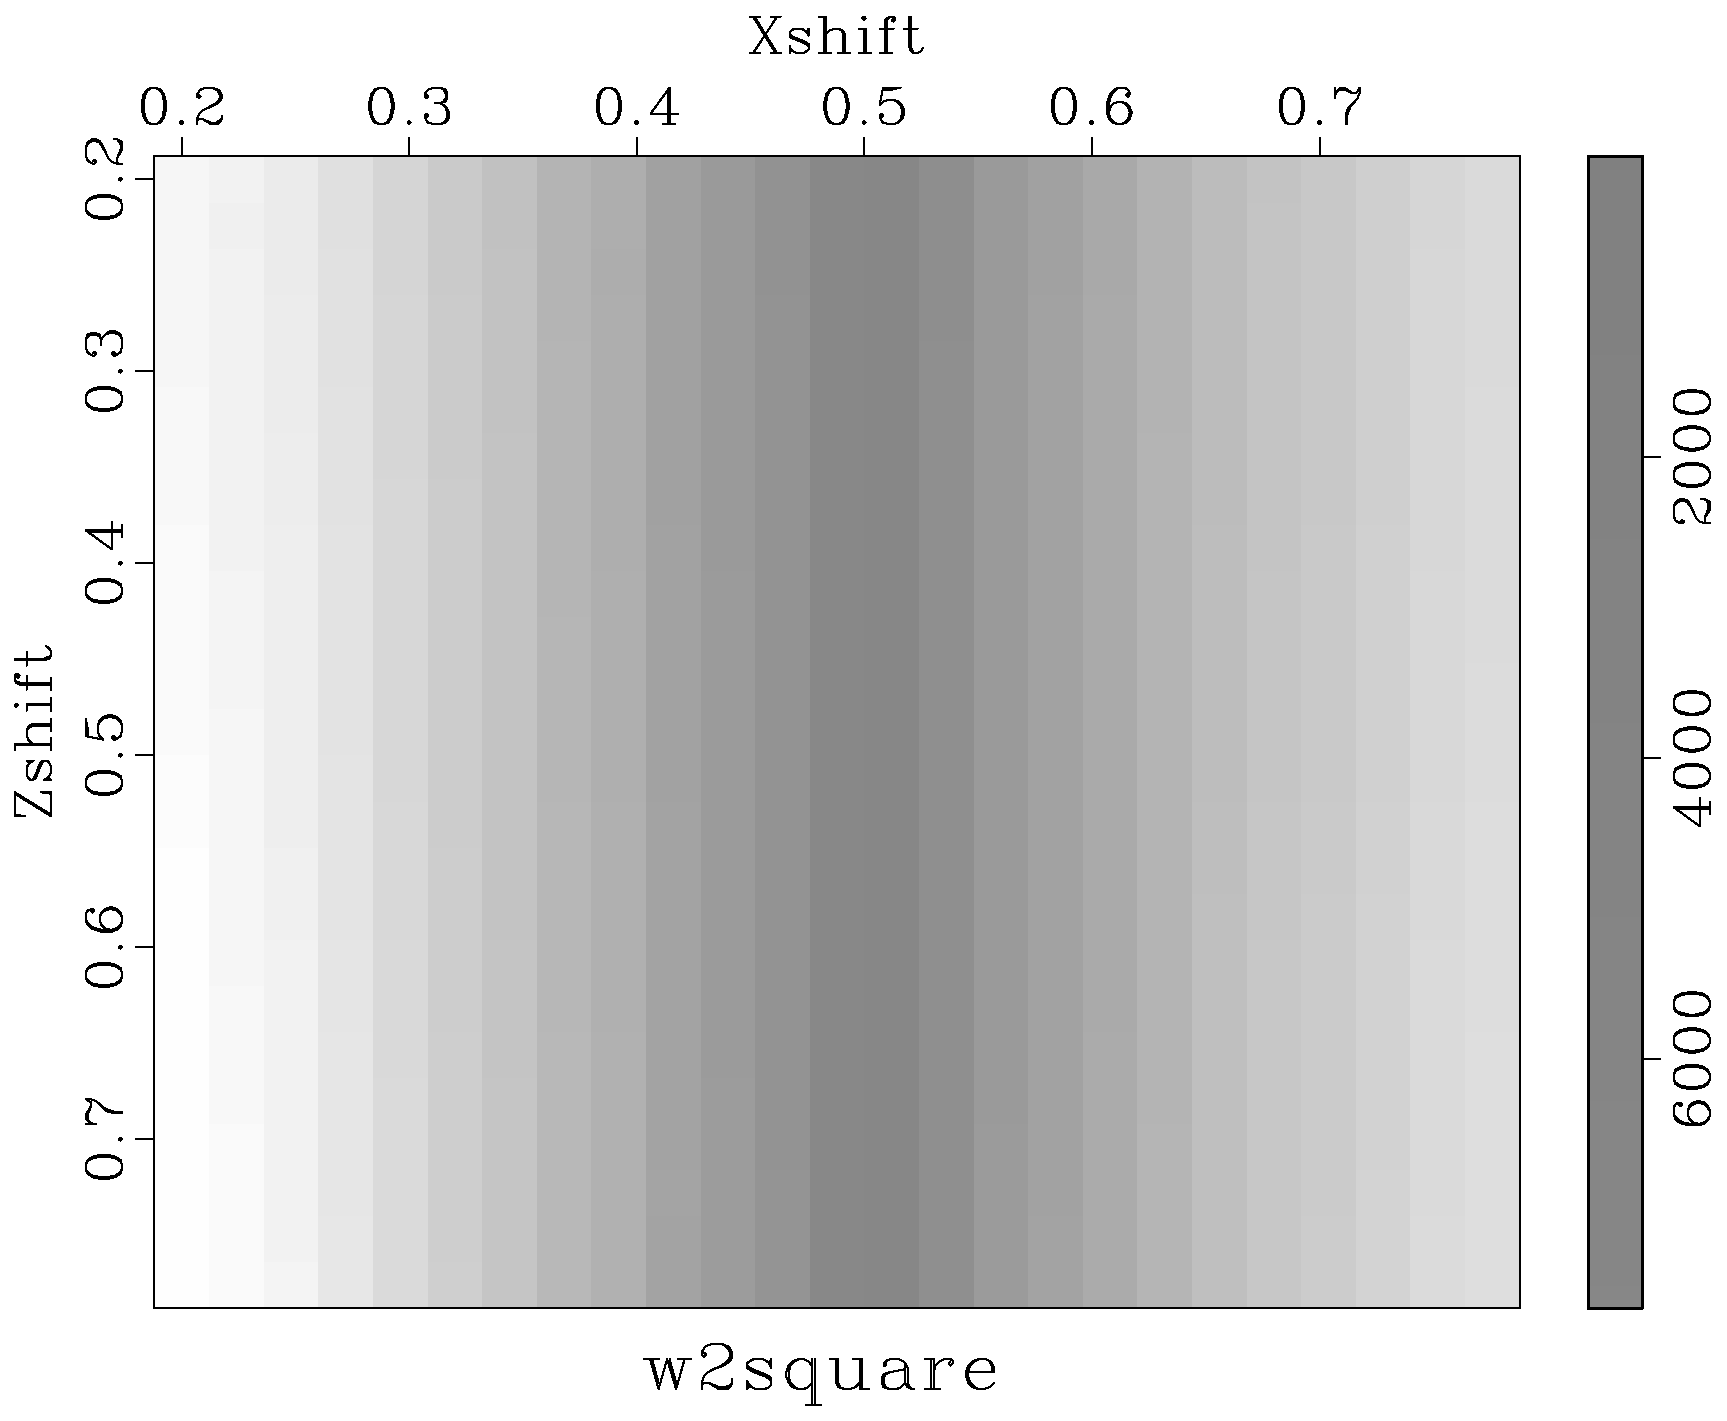
\includegraphics[width=0.5\textwidth]{Fig/fulldist2.pdf}
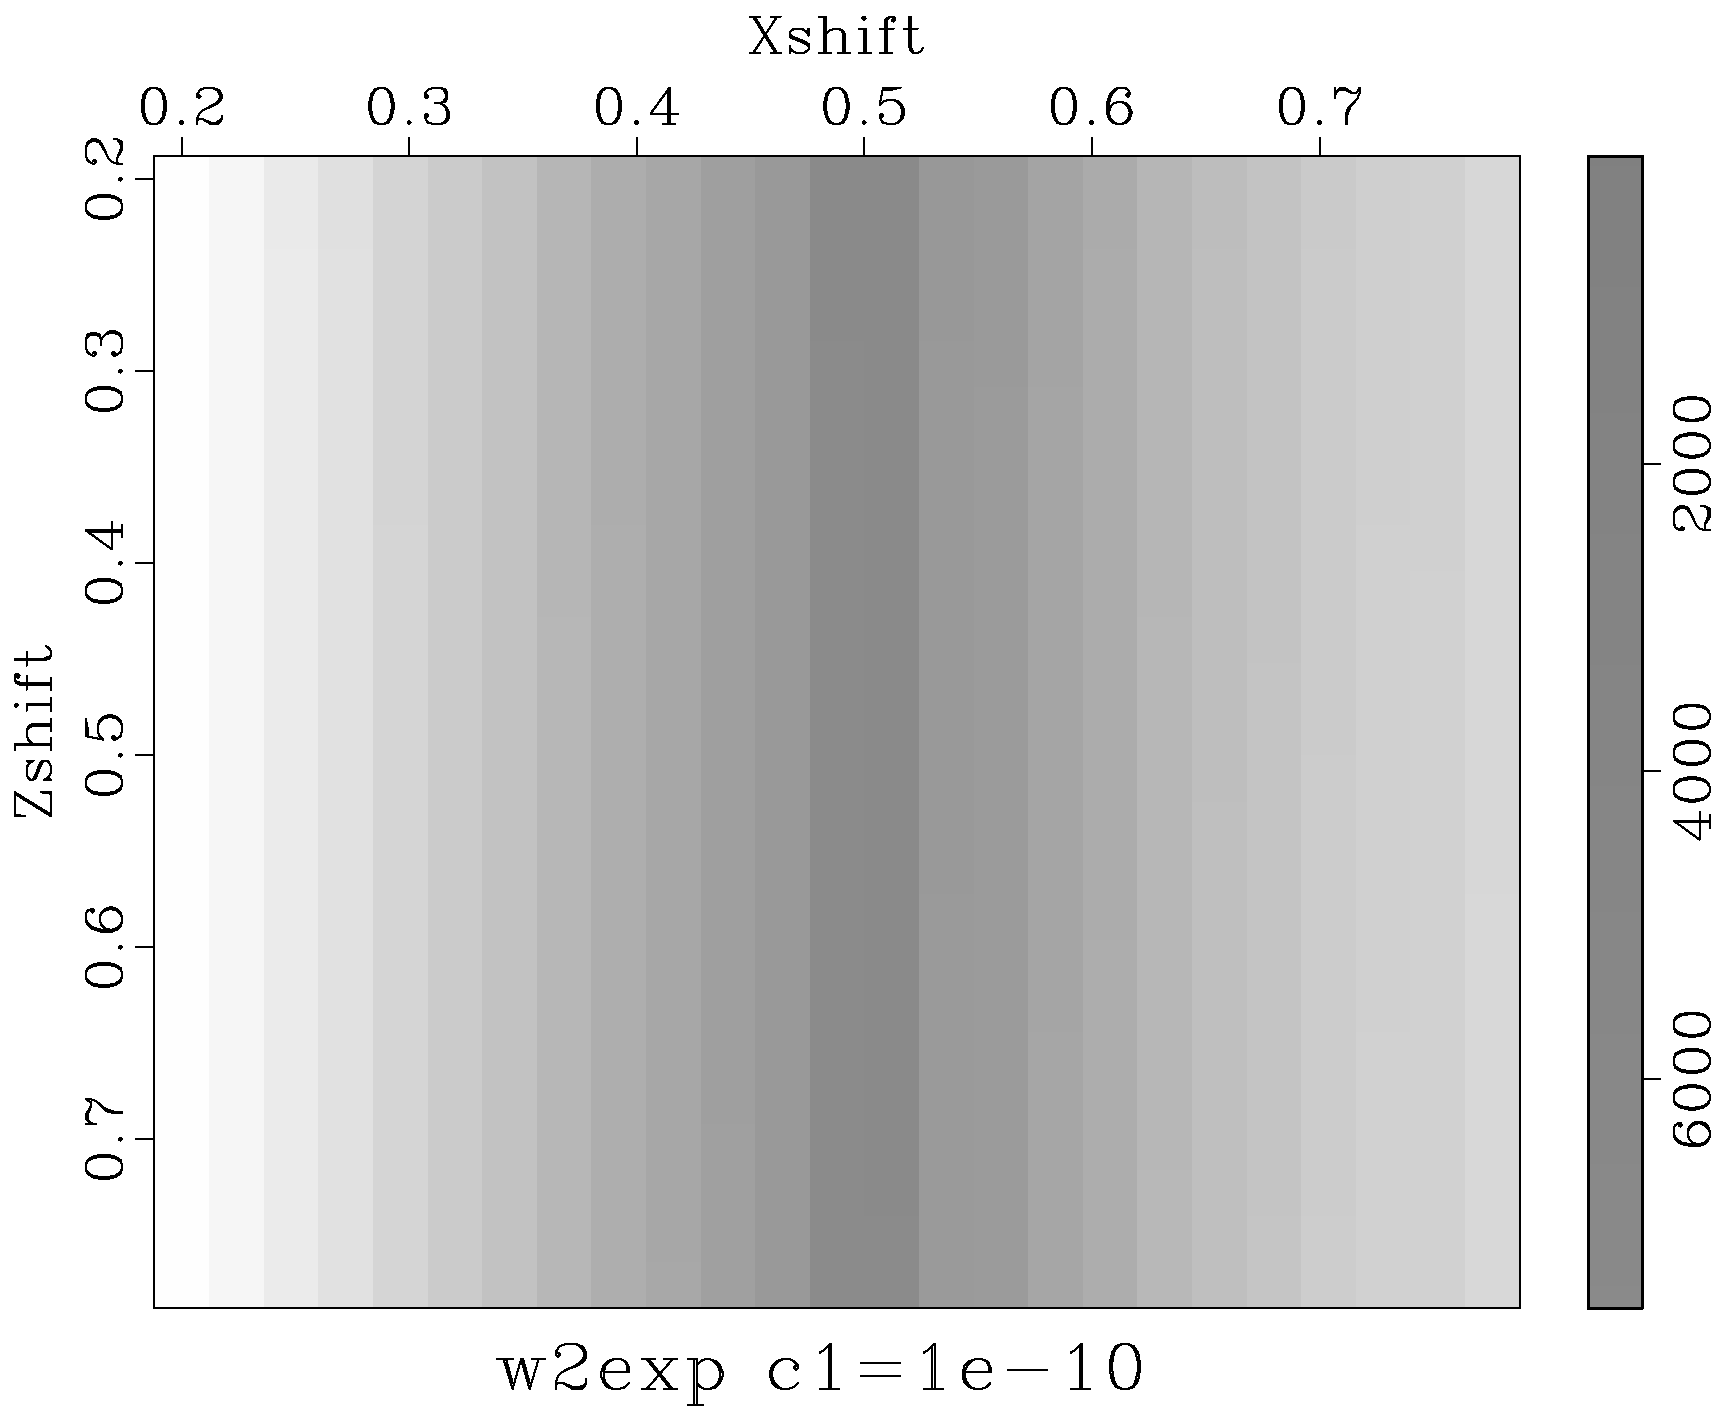
\includegraphics[width=0.5\textwidth]{Fig/fulldist3.pdf}
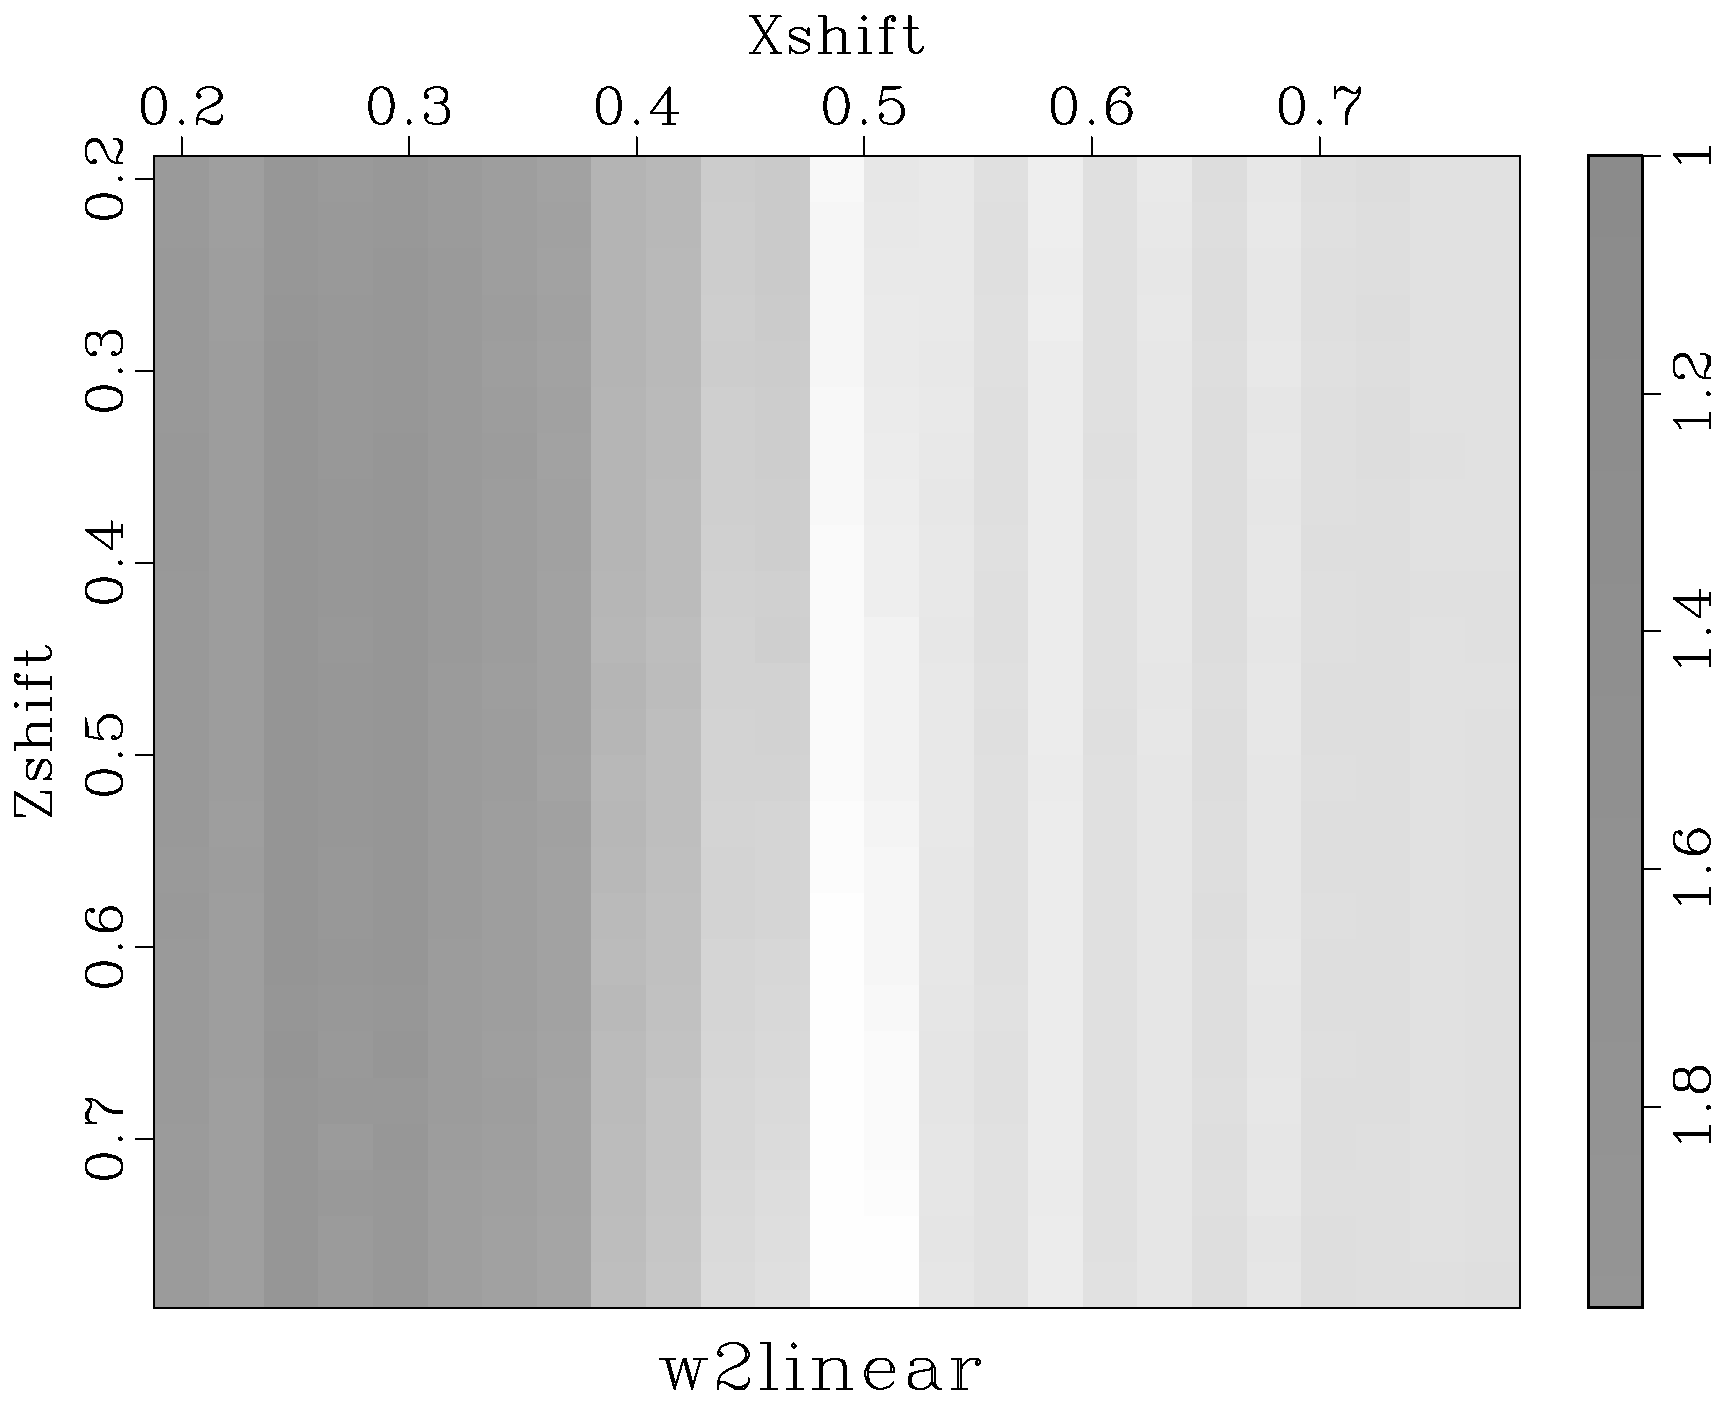
\includegraphics[width=0.5\textwidth]{Fig/fulldist4.pdf}
\caption{Optimization landscapes for various renormalization methods and their comparison with $L^2$.}
\label{fig:iaspopt}
\end{figure}

\section{Conclusions}
We demonstrate that optimal transport translates well to elastic source inversion. However, despite the general lack of oscillations in the optimization landscape as compared to $L^2$, we noticed that the landscape is relatively flat near the optimum. While some renormalization procedures worked better than others, this flatness was common to all of these methods. Renormalization destroys amplitude information, and this may be the reason for this flatness near the optimum. In short, optimal transport may successfully capture the geometry but not the amplitudes. This loss of amplitude information may be helped with the introduction of unnormalized optimal transport (\cite{gangbo2019unnormalized}) or the Wasserstein-Fisher-Rao metric (\cite{zhou2018wasserstein}), albeit at greater computational cost. 

\section{Further Reading}
For a review of misfit comparisons for FWI, we refer the reader to (\cite{brossier2010data}) and Chapter 11 of (\cite{fichtner2010full}). For a review of optimal-transport misfits for FWI, we refer to (\cite{metivier2022review}).  


\bibliographystyle{seg}  % style file is seg.bst
\bibliography{ref}

\end{document}

